The robot was built following a standard differential drive configuration (XXXX reference) because of an easier control (e.g.: rotate around it's center point without moving). A picture of the robot can be seen in Figure \ref{fig:robotPic}.

\begin{figure}[h]
        \centering
        \begin{subfigure}[b]{0.45\linewidth}
        \centering
                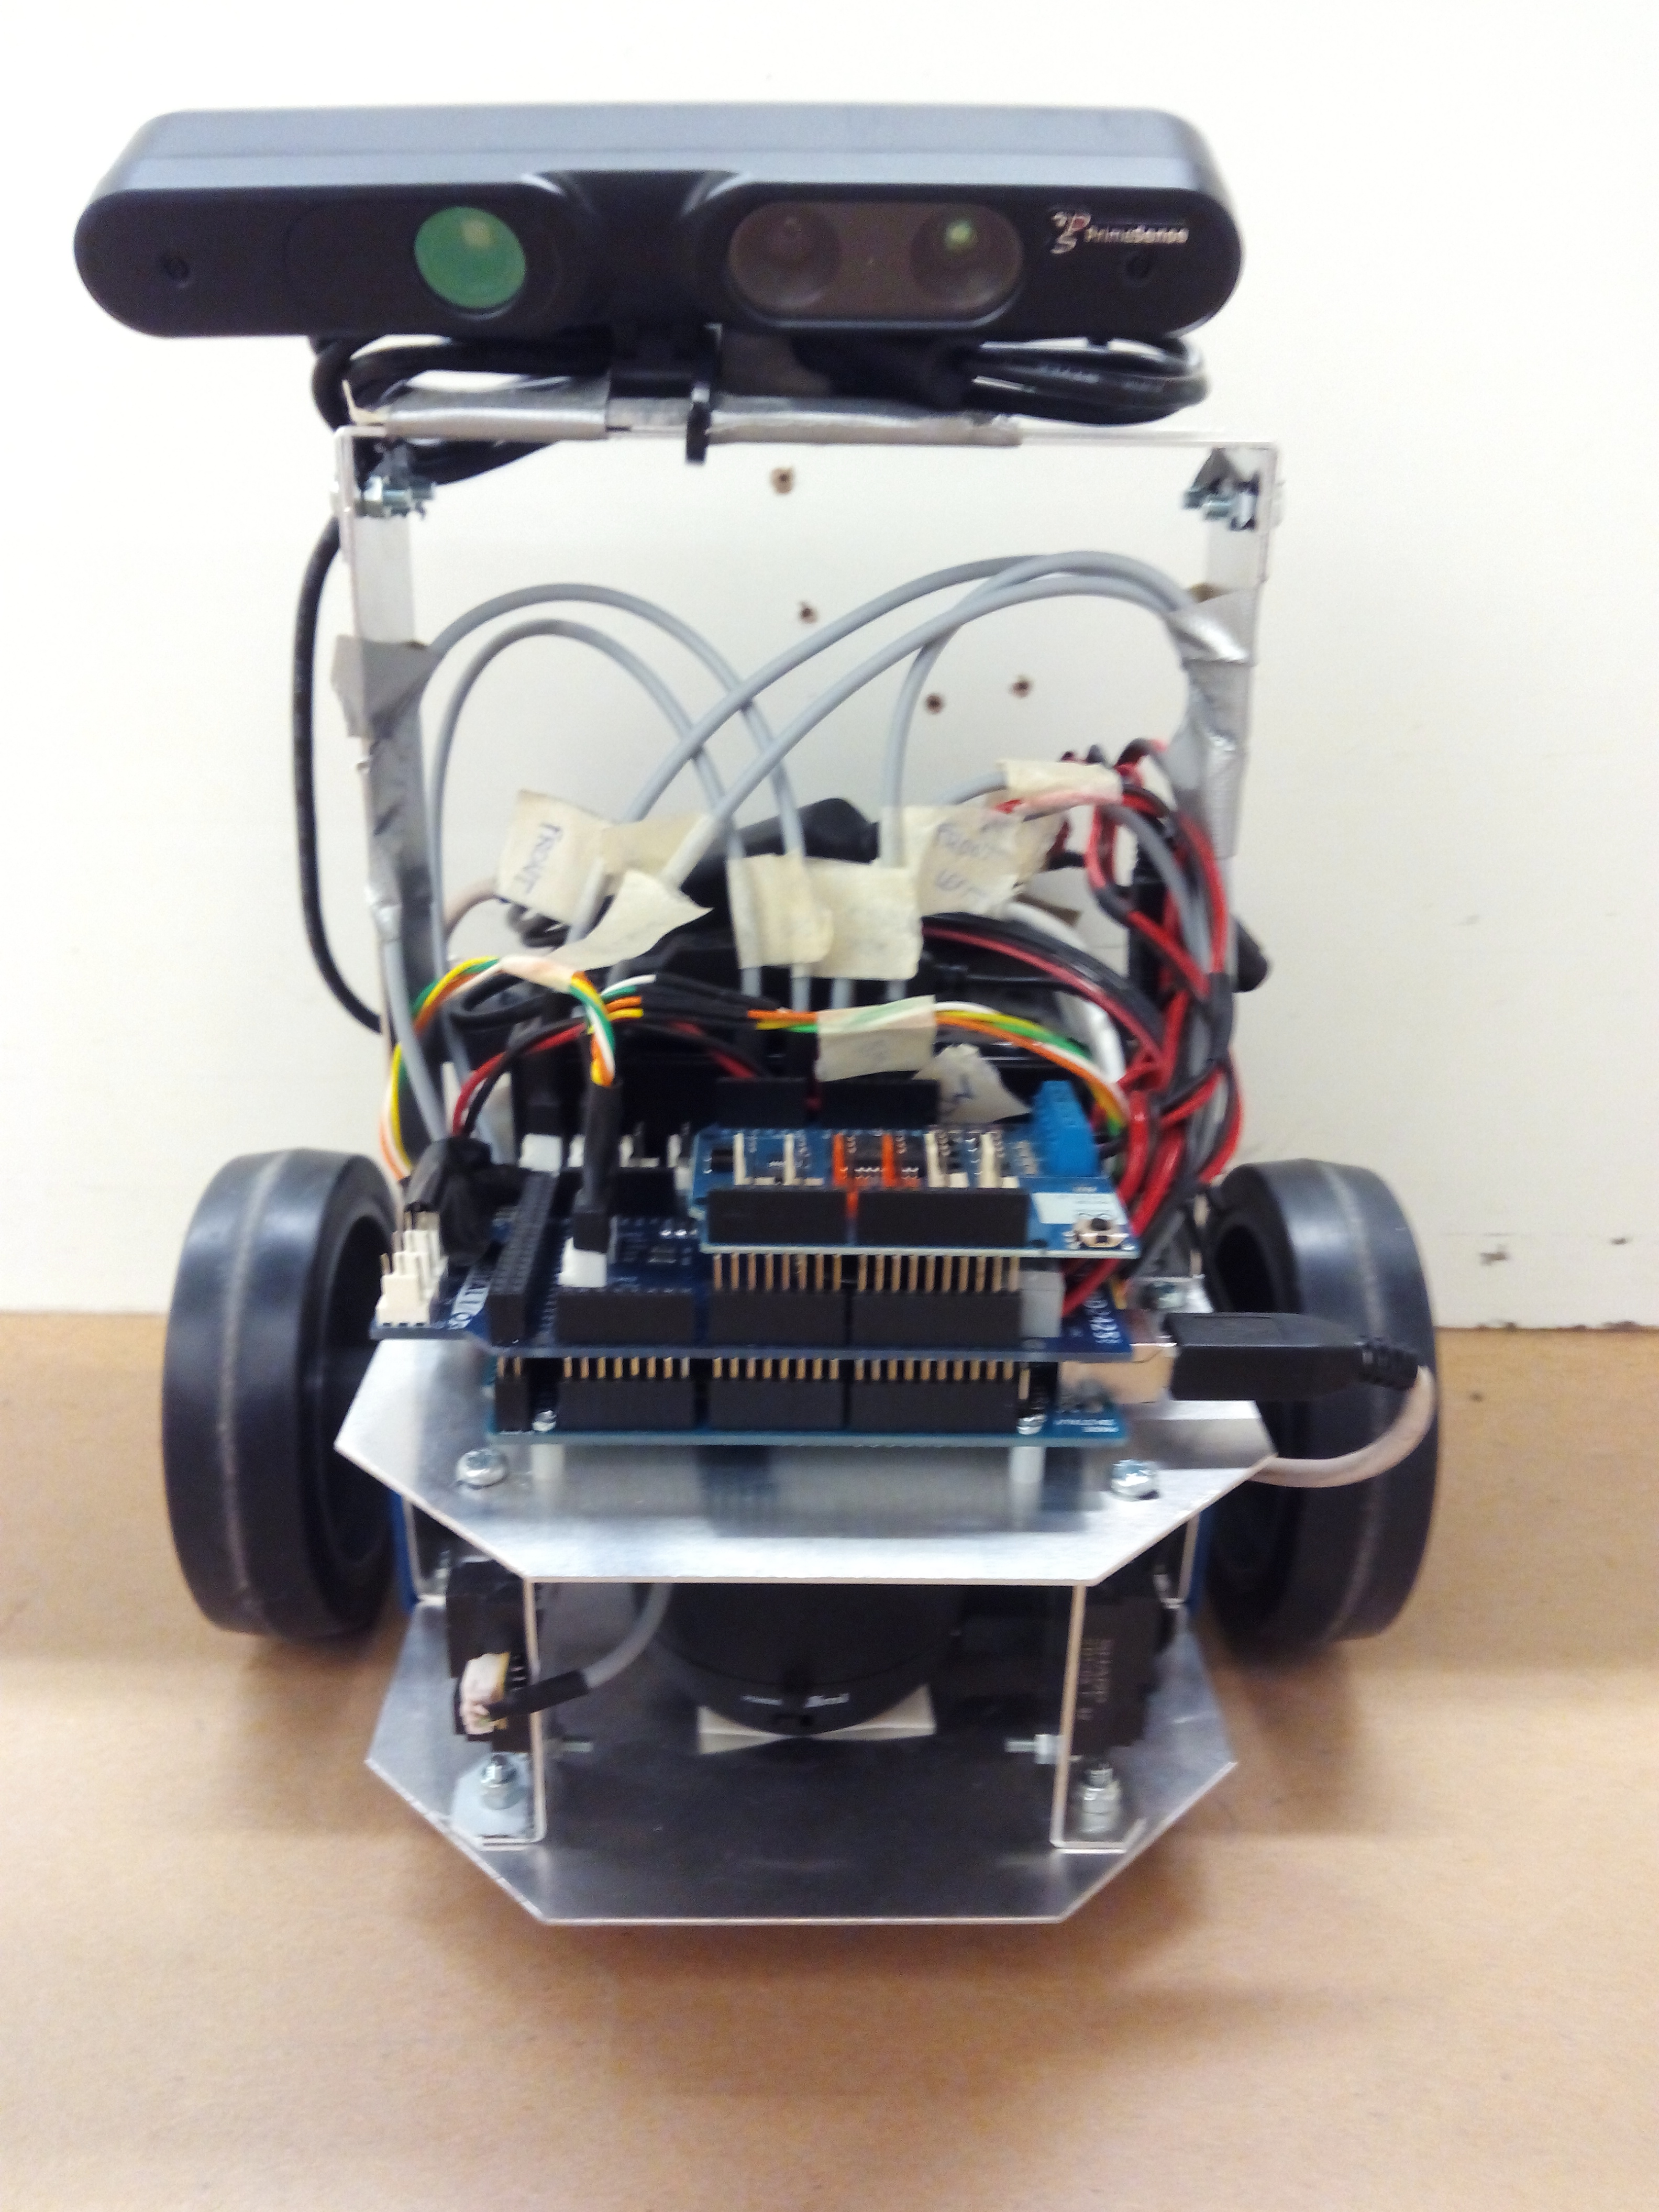
\includegraphics[height=5cm]{figures/front.jpg}
		\caption{Front view}
        \end{subfigure}
        \begin{subfigure}[b]{0.45\linewidth}
        \centering
                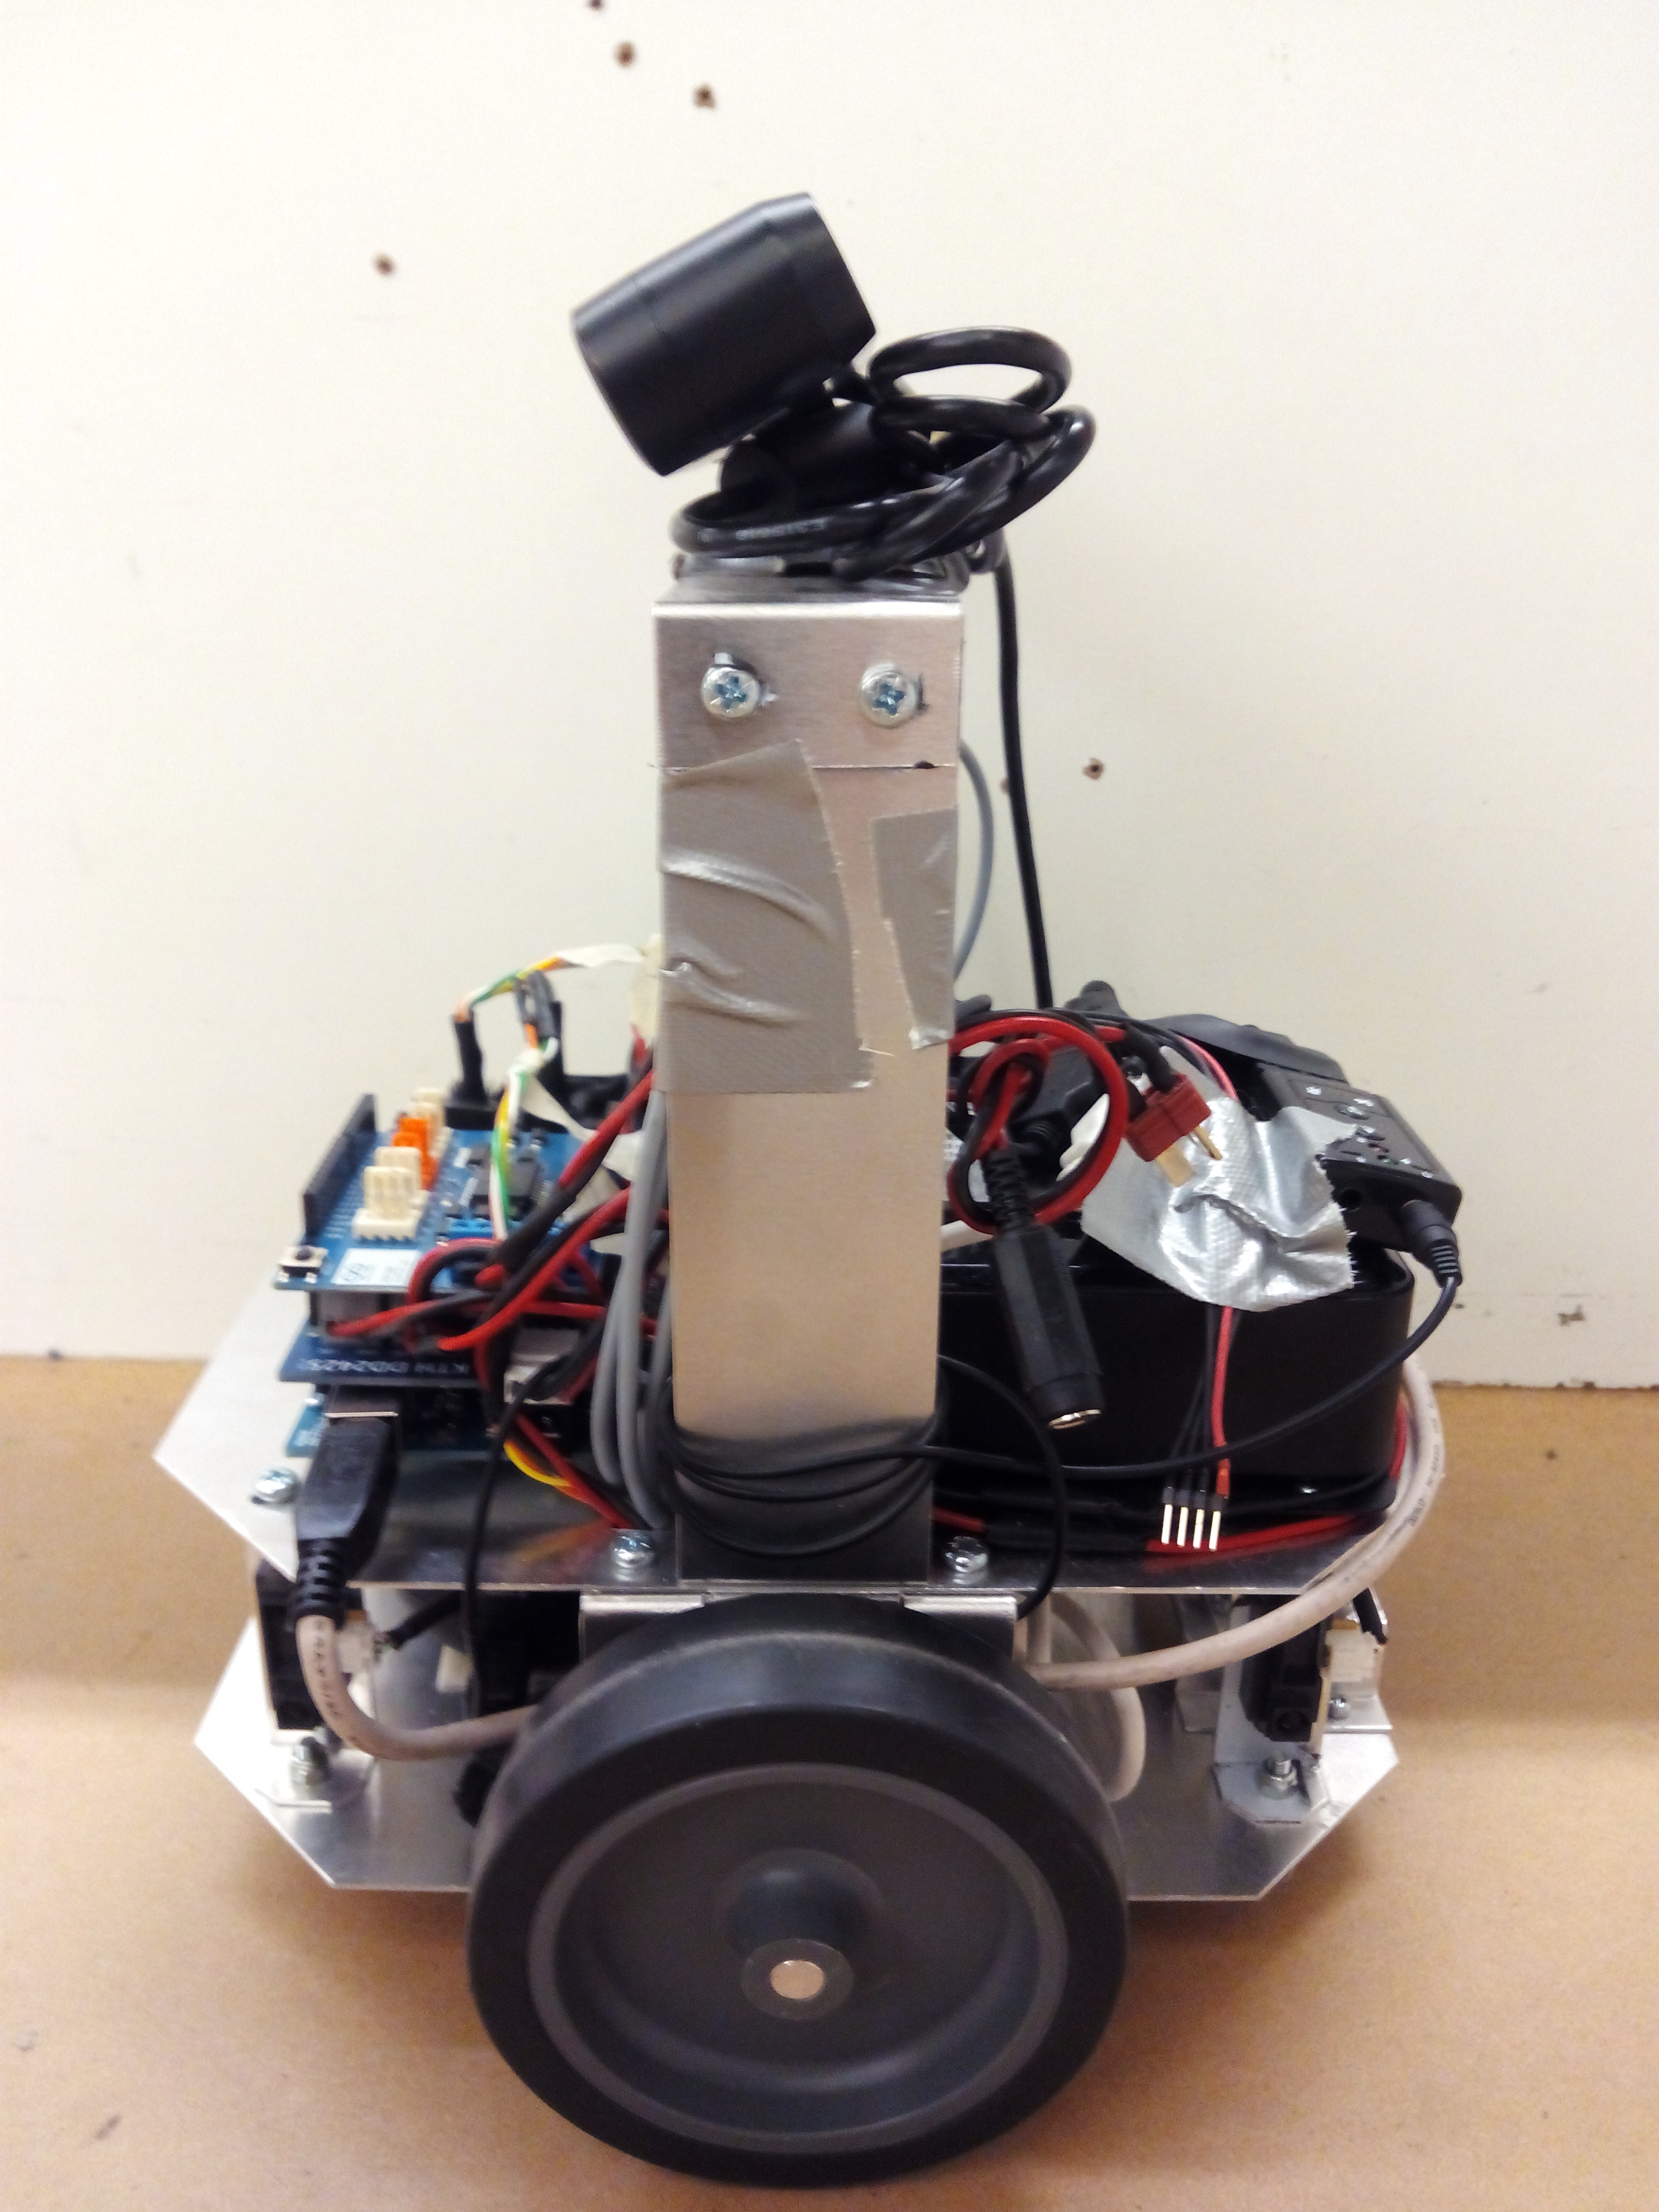
\includegraphics[height=5cm]{figures/side.jpg}
                \caption{Side view}
        \end{subfigure}
        \caption{Pictures of the robot}
                \label{fig:robotPic}
\end{figure}


The dimensions are 23 cm x 23 cm wide and long (including wheels) and 29 cm high. Two aluminium plates are connected with four pillars in order to create two floors. On the first floor are located motors, the battery and speaker whereas on the second floor the NUC and the Arduino sandwich can be found. For camera there is pillar which raises it high enough so it reaches 29 cm height. This is required in order to get depth information, which requires a minimum distance of 35 cm from the camera. The IMU is located at the center of the robot, under the second plate, as well as the long range IR sensors looking forward and backwards. The short range IR sensors are located on the pillars which connect first and second floor, with the aim of performing wall following. This is clarified with schematic \ref{fig:schematic}.